%% LyX 1.3 created this file.  For more info, see http://www.lyx.org/.
%% Do not edit unless you really know what you are doing.
\documentclass[english,12pt,a4paper,twoside]{article}
\usepackage{times}
%\usepackage{algorithm2e}
\usepackage{url}
\usepackage{bbm}
\usepackage[T1]{fontenc}
\usepackage[latin1]{inputenc}
\usepackage{geometry}
%\geometry{verbose,letterpaper,tmargin=2.5cm,bmargin=3cm,lmargin=3cm,rmargin=3cm}
\usepackage{rotating}
\usepackage{graphicx}
\usepackage{amsmath, amsthm, amssymb}
\usepackage{setspace}
\usepackage{lineno}
\usepackage{hyperref}
\usepackage{bbm}

%\usepackage{xcolor,framed}
%\colorlet{shadecolor}{blue!10}
%\begin{shaded}blabla\end{shaded}

%\usepackage{xr}
%\externaldocument{PRS-supp}

%\linenumbers
%\doublespacing
\onehalfspacing
%\usepackage[authoryear]{natbib}
\usepackage{natbib} \bibpunct{(}{)}{;}{author-year}{}{,}


%Pour les rajouts
\usepackage{xcolor}

\usepackage{dsfont}
\usepackage[warn]{textcomp}
\usepackage{adjustbox}
\usepackage{multirow}
\usepackage{graphicx}
\graphicspath{{figures/}}
\DeclareMathOperator*{\argmin}{\arg\!\min}

\let\tabbeg\tabular
\let\tabend\endtabular
\renewenvironment{tabular}{\begin{adjustbox}{max width=0.75\textwidth}\tabbeg}{\tabend\end{adjustbox}}

\makeatletter

%%%%%%%%%%%%%%%%%%%%%%%%%%%%%% LyX specific LaTeX commands.
%% Bold symbol macro for standard LaTeX users
%\newcommand{\boldsymbol}[1]{\mbox{\boldmath $#1$}}

%% Because html converters don't know tabularnewline
\providecommand{\tabularnewline}{\\}
\definecolor{clumping}{HTML}{38761D}
\definecolor{thresholding}{HTML}{1515FF}
%<span style="color:#38761D">Clumping</span> + <span style="color:#1515FF">Thresholding</span>

\usepackage{babel}
\makeatother


\begin{document}

\section{Conclusion and Discussion}

\subsection{Summary of my work}

The first part of my work has consisted in developing tools to easily analyze genotype matrices.
There are different software using different input formats so that they are sometimes difficult to use in concordance in the same analysis.
These software are of tremendous utility for the research community because they efficiently implement some of the validated analyses that are used in genetics, such as performing GWAS or heritability estimation.
Yet, if you want to do some exploratory analysis, looking at new ideas, modifying the code a little, it is practically impossible to do so.
I understood that I would need some kind of standard matrix format if I wanted to use simple code for explanatory analyses and to develop new ideas.
So, I started to develop R package bigsnpr. There is no better way for understanding methods than to implement them. 
At some point, I realized that lots of methods I was using and reimplementing for the on-disk matrix format was just some standard statistical tools that would be useful for other fields too. 
So, I put all these functions (PCA, multiple association tests, numerical summaries, matrix products, etc.) in another R package called bigstatsr that can be used by other people outside the field of genetics. 
Hopefully, this package will become useful for many people as data are getting larger in other fields too. 
I have spent a lot of time documenting, testing and optimizing the code in these two R packages. 
For example, you can now do an association analysis for a continuous outcome in no time thanks to the use of some linear algebra tricks (see the Appendix).
I have also spent some time exploring some genotype datasets and found for example that standard software for computing PCA such as PLINK and FastPCA sometimes are not accurate enough, i.e.\ that the approximation they use does not give the same results as when using an exact PCA implementation. Moreover, I have found that one should be extra careful about the SNPs that are used in PCA if they do not want to capture something else than population structure, such as LD structure\footnote{\url{https://privefl.github.io/bigsnpr/articles/how-to-PCA.html}}; I developed the ``autoSVD'' to detect those SNPs automatically and remove them.

Then, I developed some efficient implementation of penalized (linear and logistic) regressions. 
Two efficient implementations were already available for these models, but those implementations did not scale well with the very large datasets we have in the field. For example, they could not be used to analyze the UK Biobank genotyped data of 500K individuals and 800K SNPs. 
It is now possible to do so with the implementation we provide in package bigstatsr. 
The difference in computation time resides mainly in the use of some early stopping criterion in our implementation. We also provide a way to choose the two hyper-parameters of the elastic net regularization so that the user does not have to choose them arbitrarily or by implementing a cross-validation framework themself.
We extensively compared the predictive performance of our implementation of penalized regressions with standard methods such as C+T, where SNP effects are learned independently before being combined using heuristics.
We showed that for large sample sizes, penalized regressions are able to capture very small effects and that prediction is improved as compared to C+T.
For example, we are able to predict 43\% of the variance in height, which represents almost all heritability of height that can be captured by standard genotyping chips \cite[]{yang2010common,accuheight2018}.  

Finally, we focused on developing a predictive method that uses summary statistics. We first made it possible to derive the widely used C+T method for many hyper-parameters, using an efficient implementation. 
We showed that choosing over a wider range of hyper-parameter values as compared to the current practice of using C+T could substantially improve predictive performance of C+T.
We then proposed to stack all those C+T predictors instead of choosing the best one. Stacking corresponds to finding an optimal combination of different predictors in order to get higher predictive performance than any single of these predictors. 
We called this method SCT, which stands for Stacked Clumping and Thresholding.
We showed that when using external summary statistics and the UK Biobank data, we could substantially improve prediction over any C+T model.

Thus, overall we developed tools to analyze large matrices, especially genotype matrices, possibly in dosage format.
We then proposed two methods for building polygenic predictive models, one based on individual-level data (that could use summary statistics to prioritize SNPs in the model), and one based on large summary statistics and individual-level data.
Those methods provide ones of the currently best predictive performance for many diseases and traits.   


\subsection{Problem of generalization}

Polygenic Risk Scores (PRS) might become a central part in precision medicine. For now, predictive performance for most complex diseases are not good enough to be used in clinical settings. 
A major concern with PRS at the moment is their problem of generalization / transferability in different populations. 
Indeed, most GWAS have included European people only (Figure \ref{fig:GWAS-ancestry}). In 2009, 96\% of individuals included in GWAS datasets were of European ancestry \cite[]{need2009next}. In 2016, still more than 80\% of those individuals were of European descent, with an increase of the inclusion of non-European participants, mostly constituted of Asian people \cite[]{popejoy2016genomics}. People from Hispanic or African ancestry are still poorly represented \cite[]{martin2019clinical}.
This poor heterogeneity in inclusion can be explained by the fact that the more diverse are the population in the data we analyze, the more possible confounders there are to account for in order to avoid spurious results \cite[]{popejoy2016genomics}. 

\begin{figure}[htpb]
\centerline{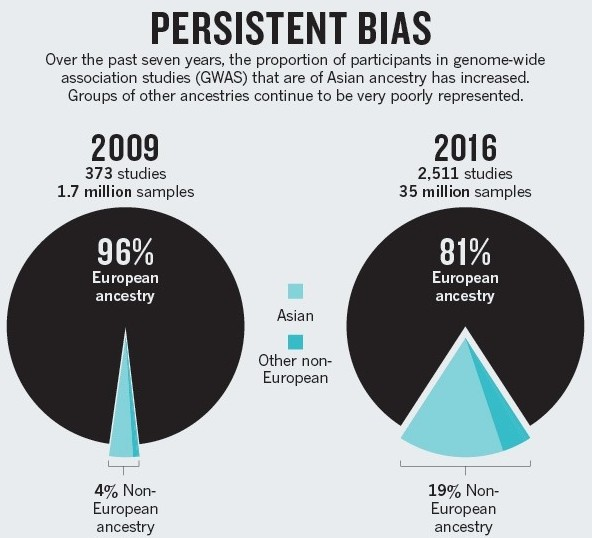
\includegraphics[width=0.6\textwidth]{GWAS-ancestry.jpg}}
\caption{Proportion of GWAS participants by ancestry. Most GWAS include mainly European people, some now include Asian people, but other ethnicities are still poorly represented. Source: \cite{popejoy2016genomics}.}
\label{fig:GWAS-ancestry}
\end{figure}

This lack of heterogeneity in inclusion of diverse populations has several problems. First, there are some SNP ascertainment bias because SNPs that are more common are more likely to be discovered in GWAS so that associated SNPs tend to have larger frequencies in European than in other populations, due to the winner's curse. 
If alleles have a frequency that is different between populations, using the corresponding effects on disease naturally introduces some shift in PRS distributions for different populations.
Second, rare variants are missed in GWAS if they are specific to some population that is not included in the association study \cite[]{martin2019clinical}. Thus, this limit the predictive ability of PRS in different populations to the one(s) included in the GWAS.
Third, it is accepted that genotyped SNPs, or even imputed SNPs, that are discovered in GWAS may not be true functional SNPs (fSNPs) having an effect on disease susceptibility. Instead, GWAS are assumed to discover SNPs that tag fSNPs (tagSNPs), i.e.\ are correlated with fSNPs. 
Yet, LD may be different between populations so that a tagSNP can have a different correlation with the corresponding fSNP. Thus, effects of these SNPs can be different and are often diluted toward zero for populations not included in the GWAS \cite[]{carlson2013generalization}. 
In conclusion, for many reasons, magnitude and frequency of effects can vary considerably between populations, and these differences are larger when populations are more genetically distant such as African population with either European or Asian populations.
These differences in prediction between populations are two-fold (Figures \ref{fig:dist-shift} and \ref{fig:pop-pred}): distributions of PRS are shifted and prediction within each distribution is also reduced \cite[]{vilhjalmsson2015modeling,martin2019clinical}.

\begin{figure}[htpb]
\centerline{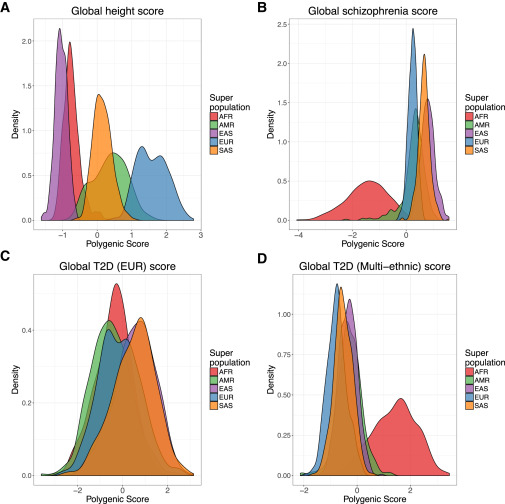
\includegraphics[width=0.6\textwidth]{pred-pops.jpg}}
\caption{Distributions of Polygenic Risk Scores (PRS) for many populations and phenotypes (T2D: type 2 diabetes). Source: \cite{martin2017human}.}
\label{fig:dist-shift}
\end{figure}

\begin{figure}[htpb]
\centerline{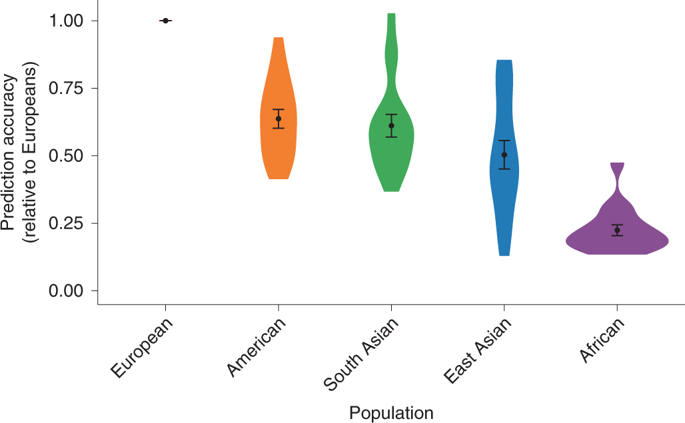
\includegraphics[width=0.7\textwidth]{pop-pred-reduced.png}}
\caption{Prediction accuracy relative to European-ancestry individuals across 17 quantitative traits and 5 continental populations in the UK Biobank data \cite[]{bycroft2017genome}. Source: \cite{martin2019clinical}.}
\label{fig:pop-pred}
\end{figure}


Several solutions have been proposed to partially correct for the differences of prediction between populations. First, \cite{martin2017human} proposed to mean-center PRS for each population, yet this would require an accurate way to assess ancestry and would not work for admixed people, e.g.\ one person with an African father and an European mother \cite[]{reisberg2017comparing}.
Second, it has been suggested to include more diverse population in GWAS \cite[]{pulit2010multiethnic}. Indeed, new associations can be found if the frequency is higher in an under-represented population. 
It would be also possible to fine-map fSNPs in common for multiple populations so that their effects generalize better to any population, irrespective of LD \cite[]{carlson2013generalization,finemap,wojcik2018page}.
Finally, statistical methods are being developed to use large European GWAS in conjunction with smaller data from another population in order to leverage both the discoveries from the large dataset and the specificities of the smaller dataset \cite[]{marquez2017multiethnic,coram2017leveraging}.


\subsection{Looking for missing heritability in rare variants}

Missing heritability, i.e.\ the gap between heritability estimations from current GWAS studies and from family studies, could reside in rare variants.
Indeed, for height and colorectal cancer, it has been shown that estimations of heritability from GWAS data could recover almost all heritability when a large proportion of low-frequency variants was present in the data \cite[]{yang2015genetic,huyghe2019discovery,wainschtein2019recovery}.
However, actual findings of significantly associated variants of low-frequency are scarce. 
For example, a GWAS of height including more than 700K individuals found 83 associated variants with allele frequencies between 0.1\% and 4.8\%, with effects up to 2 cm per allele \cite[]{marouli2017rare}. Yet, these 83 variants together accounts for only 1.7\% of the total heritability of height. 
In other large studies, one for coronary artery disease and one for type 2 diabetes, there was little evidence of low-frequency variants with large effects \cite[]{nikpay2015comprehensive,fuchsberger2016genetic}.

Associations of rare variants with traits are difficult to find for two reasons. 
First, it is very difficult to impute low-frequency variants with a good quality if using for example a small reference panel such as the 1000 genomes \cite[]{nikpay2015comprehensive}. There is now a reference panel of 32,000 individuals that is used to accurately impute variants with allele frequencies as low as 0.1\% \cite[]{mccarthy2016reference}. Ongoing large-scale projects, such as the Trans-Omics for Precision Medicine (TOPMed) programme, are expected to produce reference panels 
of more than 100,000 individuals \cite[]{taliun2019sequencing}.
This large reference panel is European specific, which means that imputing data from other ancestries is more difficult. This is a problem because, one way to discover and accurately estimate the effect of a rare variant is to look for it in a population in which its allele frequency is larger \cite[]{moltke2014common,minster2016thrifty}. 
Indeed, the power of association studies is dependent on the variance explained by a locus and its frequency; for example, for a disease that affects 1\% of the population, we have the same power to detect a risk locus of 50\% frequency and odds ratio of 1.1 as we do for a risk locus of 0.1\% frequency and odds ratio of 2.9 \cite[]{wray2018common}.

The second reason for which rare variant associations are difficult to find is that sequencing technologies are more expensive than genotyping and imputation. Currently, studies have mostly focused on whole exome sequencing (WES) because it is cheaper than whole genome sequencing (WGS). 
Indeed, the exome is where the effect sizes of variants are expected to be larger and where discoveries are likely to be more immediately actionable \cite[]{zuk2014searching}. 
Yet, sample sizes of sequencing studies remain small and special considerations and challenges arise when testing rare frequency variants from these studies \cite[]{auer2015rare}.
Thus, sample size is the limiting factor in variant discovery, not genotyping technology \cite[]{wray2018common}. 
It is probably the limiting factor in prediction too.

\subsection{Looking for missing heritability in non-additive effects}

Knowledge about biological pathways and gene networks implies that epistasis (gene interactions) might be important to consider \cite[]{hill2008data}. 
Apart from explaining missing heritability, genetic interactions could also create phantom heritability, i.e.\ could make current estimation of heritability upward biased \cite[]{zuk2012mystery}.
There have been some findings of interaction between loci, but mainly for autoimmune diseases where there are strong effects in regions of chromosome 6 that have an effect on the autoimmune system \cite[]{lenz2015widespread,goudey2017interactions}.
Yet, these interaction effects explain little to phenotypic variance as compared to additive effects \cite[]{lenz2015widespread}.
In general, data and theory point to mainly additive genetic variance \cite[]{hill2008data}.

Moreover, interactions are challenging to find for two reasons, and dedicated methods to epistasis detection have been implemented \cite[]{niel2015survey}. First, it is analytically impractical to search for such interaction effects because it would require testing more than 100 billion pairs of variants, even for a small genotyping array. Second, because of this huge number of tests, correction for multiple testing allows the detection of highly significant interactions only.

Finally, even if we find such interaction effects, they are unlikely to dramatically improve risk prediction for complex diseases, but could still provide insights into their ethiology \cite[]{aschard2012inclusion}. 
Moreover, due to differences in effect sizes and LD between populations, epistatic effects are even more unlikely than additive effects to replicate to different populations  \cite[]{hill2008data,visscher201710}.

\subsection{Integration of multiple data sources}

There are many genetic data out there. Some large individual-level data such as the UK biobank are available \cite[]{bycroft2017genome}. When GWAS data is not publicly available, summary statistics are often publicly shared instead. 
Usually, predictive models are based on either individual-level data (e.g.\ penalized regression) or summary statistics (e.g.\ C+T).
Building models that combine both individual-level data and summary statistics, possibly including different populations, is necessary to increase predictive power.
We started to do this by implementing the SCT method in our latest paper, where we combine several summary statistics based predictors using large individual-level data.
Alike with the adaptive lasso \cite[]{zou2006adaptive}, one could also think of penalizing SNPs differently in individual-level data methods, applying a penalization factor to each SNP based on their significance in external summary statistics.

Human diseases are inherently complex and governed by the complicated interplay of several underlying factors \cite[]{dey2013integration}.
For a trait or a disease, prediction based on genetic data only is ultimately capped by heritability.
Therefore, prediction must integrate other types of data if we want to predict beyond the limit of heritability (Figure \ref{fig:data-layers}).
For example, DNA methylation data can accurately predict age of any tissue across the entire life course \cite[]{horvath2013dna,horvath2018dna}, gene expression profiles enable to gain a broad picture of the genomic response to environmental perturbation \cite[]{gibson2008environmental} and microbiota can also be an important ``environmental'' factor to take into account \cite[]{backhed2004gut}. 
Yet, integrating variables with different formats, types, structure, dimensionality and missing values is a challenging problem \cite[]{dey2013integration}.
One could integrate genetic data with clinical data. For example, \cite{inouye2018genomic} designed a polygenic risk score (PRS) with higher discriminative ability for coronary artery disease than any of 6 conventional risk factors (smoking, diabetes, hypertension, body mass index, high cholesterol and family history).
Using this PRS with all 6 conventional risk factors increases discriminative ability as compared to using the PRS only or the 6 factors only.
Moreover, electronic health records (EHR) make possible to integrate large biobank datasets with large clinical, environmental and phenotypic information \cite[]{roden2016integrating}.
%Three different approaches for data integration are presented in figure \ref{fig:int-data} \cite[]{dey2013integration,zitnik2019machine}.

\begin{figure}[htpb]
\centerline{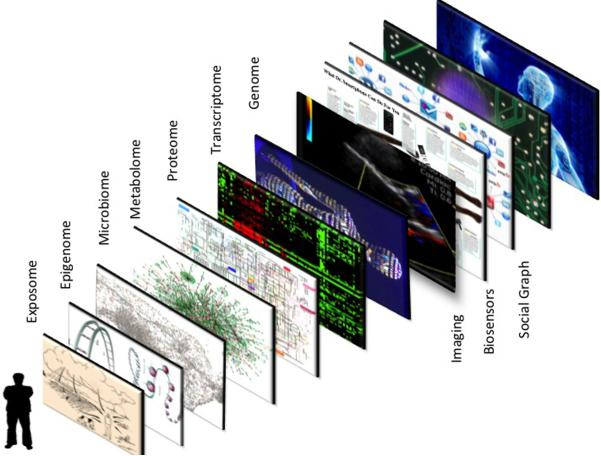
\includegraphics[width=0.7\textwidth]{data-layers}}
\caption{Geographic information system of a human being. The different layers of data available for an individual. Source: \cite{topol2014individualized}.}
\label{fig:data-layers}
\end{figure}


\subsection{Future work}

I will probably continue to work in the field of Predictive Human genetics. I am currently visiting the National Center for Register-based Research (NCRR) in Aarhus, Denmark. Researchers there are mostly epidemiologists using some national registers where they have information on all Danes over decades. Most of their work is funded to look at psychiatric disorders and they are now interested in how genetics influence psychiatric conditions. It is a good opportunity to work on a large national biobank dataset with Bjarni Vilhj\'almsson.

I would be interested in looking at many things. 
First, I think investigating which method works best in which scenario is of great interest for the field. 
Many scenarios could involve different sample sizes of summary statistics and individual-level data, but also training and prediction in different populations.
Such work could be useful to make some guidelines about which method to use in which situation. For example, individual-level data methods often work best when large individual-level data are available, but what about predicting in a different population where only smaller datasets are available?
Second, it would be interesting to account for age in the prediction, for example extending with Cox regression the methods I implemented. Many diseases such as cancer, heart diseases and Alzheimer's disease have an age component; modeling this age component and accounting for right censoring (people who might develop disease later) should increase predictive performance and usefulness of models.
Third, I would like to investigate more about imputation. At the moment, imputed data is taken for granted. How to properly account for imputation accuracy in association testing (using e.g.\ multiple imputation) and in predictive models? 

Finally, other ideas could be to investigate how we can integrate many sources of information such as functional annotations, looking at many phenotypes at once, or to distinguish between two diseases with similar symptoms using polygenic risk scores (e.g.\ diabetes).

\newpage

\bibliographystyle{natbib}
\bibliography{refs}

\end{document}
